%% ****** Start of file apstemplate.tex ****** %
%%
%%
%%   This file is part of the APS files in the REVTeX 4 distribution.
%%   Version 4.1r of REVTeX, August 2010
%%
%%
%%   Copyright (c) 2001, 2009, 2010 The American Physical Society.
%%
%%   See the REVTeX 4 README file for restrictions and more information.
%%
%
% This is a template for producing manuscripts for use with REVTEX 4.0
% Copy this file to another name and then work on that file.
% That way, you always have this original template file to use.
%
% Group addresses by affiliation; use superscriptaddress for long
% author lists, or if there are many overlapping affiliations.
% For Phys. Rev. appearance, change preprint to twocolumn.
% Choose pra, prb, prc, prd, pre, prl, prstab, prstper, or rmp for journal
%  Add 'draft' option to mark overfull boxes with black boxes
%  Add 'showpacs' option to make PACS codes appear
%  Add 'showkeys' option to make keywords appear
\documentclass[aps,pre,twocolumn,groupedaddress]{revtex4-1}
%\documentclass[aps,pre,preprint,superscriptaddress]{revtex4-1}
%\documentclass[aps,prl,reprint,groupedaddress]{revtex4-1}

% You should use BibTeX and apsrev.bst for references
% Choosing a journal automatically selects the correct APS
% BibTeX style file (bst file), so only uncomment the line
% below if necessary.
\bibliographystyle{apsrev4-1}

\usepackage{graphicx}
\usepackage{amsmath}

\begin{document}

% Use the \preprint command to place your local institutional report
% number in the upper righthand corner of the title page in preprint mode.
% Multiple \preprint commands are allowed.
% Use the 'preprintnumbers' class option to override journal defaults
% to display numbers if necessary
%\preprint{}

%Title of paper
\title{Flow Behaviour of Cubic Blue Phases in Confined Geometries}

% repeat the \author .. \affiliation  etc. as needed
% \email, \thanks, \homepage, \altaffiliation all apply to the current
% author. Explanatory text should go in the []'s, actual e-mail
% address or url should go in the {}'s for \email and \homepage.
% Please use the appropriate macro foreach each type of information

% \affiliation command applies to all authors since the last
% \affiliation command. The \affiliation command should follow the
% other information
% \affiliation can be followed by \email, \homepage, \thanks as well.
\author{O. Henrich$^{1,3}$, K. Stratford$^2$, D. Marenduzzo$^3$, P.V. Coveney$^1$ and M.E. Cates $^3$}
\affiliation{$^1$ Centre for Computational Science, University College London, UK\\$^2$ Edinburgh Parallel Computing Centre, University of Edinburgh, UK\\$^3$ School of Physics and Astronomy, University of Edinburgh, UK}

%\email[]{}
%\homepage[]{Your web page}
%\thanks{}
%\altaffiliation{}

%Collaboration name if desired (requires use of superscriptaddress
%option in \documentclass). \noaffiliation is required (may also be
%used with the \author command).
%\collaboration can be followed by \email, \homepage, \thanks as well.
%\collaboration{}

%\noaffiliation

\date{\today}

\begin{abstract}
\end{abstract}

% insert suggested PACS numbers in braces on next line
\pacs{}
% insert suggested keywords - APS authors don't need to do this
%\keywords{}

%\maketitle must follow title, authors, abstract, \pacs, and \keywords
\maketitle

% body of paper here - Use proper section commands
% References should be done using the \cite, \ref, and \label commands
\section{Introduction}
% Put \label in argument of \section for cross-referencing
%\section{\label{}}
\section{Model and Methods}

%Our approach is based on a well-established model for hydrodynamics of cholesteric liquid crystals \cite{Beris:1994,Olmsted:1999} that describes the order structure of the liquid crystal by a traceless, symmetric tensor order parameter ${\bf Q}({\bf r})$. 
%In uniaxial approximation the tensor order paramter is given by $Q_{\alpha \beta}=\langle n_\alpha n_\beta - 1/3\; \delta_{\alpha\beta}\rangle$, whereas ${\bf n}$ represents the local orientation of the liquid crystal molecules and brackets indicate mesoscopic averaging over a large number individual molecules.
%Its largest eigenvalue $\frac{2}{3}q$ with $0<q<1$ characterizes the degree of order around the corresponding axis. 
%The equilibrium properties of the system are determined by a Landau-de Gennes free energy density $f$ and the functional ${\cal F}[Q]=\int d^3{\bf r} f({\bf Q})$.
%The free energy density consists of two different parts, namely a bulk contribution $f_b$ and a gradient term $f_g$.

%\begin{eqnarray}
%f_b&=&\frac{A_0}{2}\left(1-\frac{\gamma}{3}\right) Q_{\alpha \beta}^2-\frac{A_0 \gamma}{3}Q_{\alpha \beta} Q_{\beta \gamma} Q_{\gamma \alpha}+\frac{A_0 \gamma}{4}(Q_{\alpha \beta}^2)^2\nonumber\\
%f_g&=&\frac{K}{2}(\varepsilon_{\alpha\gamma\delta} \partial_\gamma Q_{\delta\beta}+2 q_0 Q_{\alpha \beta})^2+\frac{K}{2}(\partial_\beta Q_{\alpha \beta})^2\label{eqn1}
%\end{eqnarray}

%The first term contains the bulk-free energy constant $A_0$ and the inverse temperature $\gamma$ and features a the first-order transition from the isotropic to the ordered phase at $\gamma>2.7$.
%The second part comprises the elastic contributions to the free energy due to splay-, bend- and twist-deformations and assume for simplicity that they have all the same elastic constant $K$.
%The pitch length $p$ of the cholesteric liquid crystal is related to the wavervector $q_0=2\pi/p$.
%In order to specify a thermodynamic state it is useful to introduce two dimensionless quantities, the effective temperature $\tau$ and chirality $\kappa$.
%They are given by 

%\begin{eqnarray}
%\tau&=&\frac{27(1-\gamma/3)}{\gamma}\nonumber\\
%\kappa&=&\sqrt{\frac{108 K q_0^2}{A_0 \gamma}}\nonumber,
%\end{eqnarray}

%whereas the chirality qqnatifies the ratio between gradient and bulk free energy.\\
%The equation of motion of the tensor order parameter reads

%\begin{equation}\label{}
%\left(\partial_t+ u_\alpha \partial_\alpha \right){\bf Q} - {\bf S}({\bf W},{\bf Q}) = \Gamma {\bf H}.
%\label{eqn2}
%\end{equation}

%The first term on the lefthand side of Eq.(\ref{eqn2}) is a material derivative, which describes the rate of change of a quantity moving along with the flow.
%The second term accounts for the rate of change due to velocity gradients $W_{\alpha \beta}=\partial_\beta u_\alpha$:

%\begin{eqnarray}
%{\bf S}({\bf W}, {\bf Q}) &=& (\xi {\bf A} + {\boldsymbol \Omega})({\bf Q}+\frac{\bf I}{3})\nonumber\\
%& &\hspace*{-1.5cm}+ ({\bf Q}+\frac{\bf I}{3})(\xi {\bf A}  - {\boldsymbol \Omega})-2 \xi ({\bf Q}+\frac{\bf I}{3})Tr({\bf Q W}),
%\label{eqn3}
%\end{eqnarray}

%where $Tr$ denotes the trace operation and ${\bf A}=({\bf W}+{\bf W}^T)/2$ and ${\boldsymbol \Omega}=({\bf W}-{\bf W}^T)/2$ are the symmetric and antisymmetric part of the velocity gradients, respectively.
%The molecular details of the liquid crystal such as the aspect ratio of its mesogens are embodied in the constant $\xi$, also know as the tumbling parameter.
%The righthand side relates the rate of change to the molecular field, which is a functional derivative of $\cal F$ that preserves the tracelessness of $\bf Q$.

%\begin{equation}
%{\bf H}=-\frac{\delta {\cal F}}{\delta {\bf Q}}+\frac{\bf I}{3}\, Tr\left(\frac{\delta {\cal F}}{\delta {\bf Q}}\right).
%\label{eqn4}
%\end{equation}

%The rotational diffusion constant $\Gamma$ is proportional to the inverse of the rotational viscosity $\gamma_1=2 q^2/\Gamma$.\\
%The time evolution of density and velocity are goverend by the continuity equation Eq. (\ref{eqn5}) 

%\begin{eqnarray}
%\partial_t \rho + \partial_\alpha (\rho u_\alpha)=0
%\label{eqn5}
%\end{eqnarray}

%and the Navier-Stokes equation Eq. (\ref{eqn6})

%\begin{eqnarray}
%\partial_t u_\alpha +\rho \,u_\beta \partial_\beta u_\alpha&=&\partial_\beta \Pi_{\alpha \beta}\nonumber\\
%&+&\hspace*{-2cm}\eta\, \partial_\beta \{ \partial_\alpha u_\beta + \partial_\beta u_\alpha +(1+3\frac{P_0}{\partial \rho} )\partial_\mu u_\mu \delta_{\alpha \beta})\}. 
%\label{eqn6}
%\end{eqnarray}

%At low flow rates the fluid can be considered as incompressible, so that the last term on the righthand side of Eq. (\ref{eqn6}) can be safely neglected.
%The pressure tensor reads explicitely

%\begin{eqnarray}
%\Pi_{\alpha \beta}&=&P_0-\xi H_{\alpha \gamma}\left(Q_{\gamma \beta} +\frac{1}{3} \delta_{\gamma \beta}\right)-\xi \left(Q_{\alpha \gamma} +\frac{1}{3} \delta_{\alpha \gamma}\right) H_{\gamma \beta}\nonumber\\
%&+& 2 \xi  \left(Q_{\alpha \beta} +\frac{1}{3} \delta_{\alpha \beta}\right) Q_{\gamma \nu} H_{\gamma \nu}-\partial_\alpha Q_{\gamma \nu} \frac{\delta{\cal F}}{\delta \partial_{\beta} Q_{\gamma \nu}}\nonumber\\
%&+&Q_{\alpha \gamma}H_{\gamma \beta}-H_{\alpha \gamma} Q_{\gamma \beta}.
%\label{eqn7}
%\end{eqnarray}

%It comprises the terms that give rise to an additional stress in the ordered state.
%In the isotropic state when ${\bf Q}\equiv 0$ Eq. (\ref{eqn7}) is reduced to the scalar pressure, which is constant to a very good approximation.\\ 
%The system of coupled partial differential equations is solved by means of a hybrid scheme \cite{Denniston:2004, Marenduzzo:2008} that uses a lattice Boltzmann algorithm with predictor-corrector scheme for the hydrodynamic equations (\ref{eqn5}) and (\ref{eqn6}) and a finite difference scheme for the tensor order parameter equation (\ref{eqn2}).


\section{Results and Discussion}

\begin{figure*}[h]
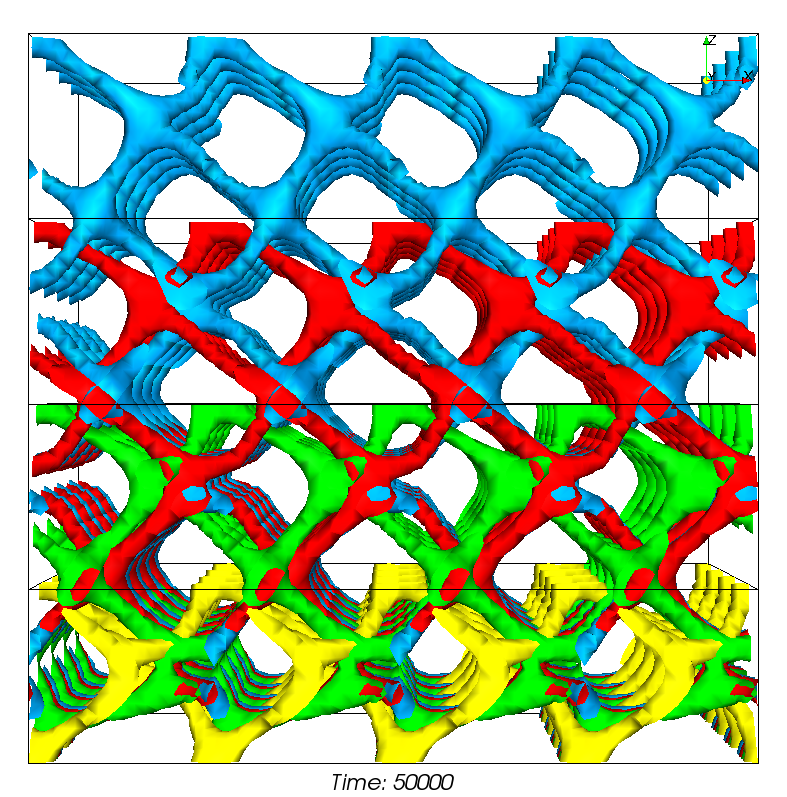
\includegraphics[width=0.245\textwidth]{disc_bp2_t-0o5_k2o0_50k.png}
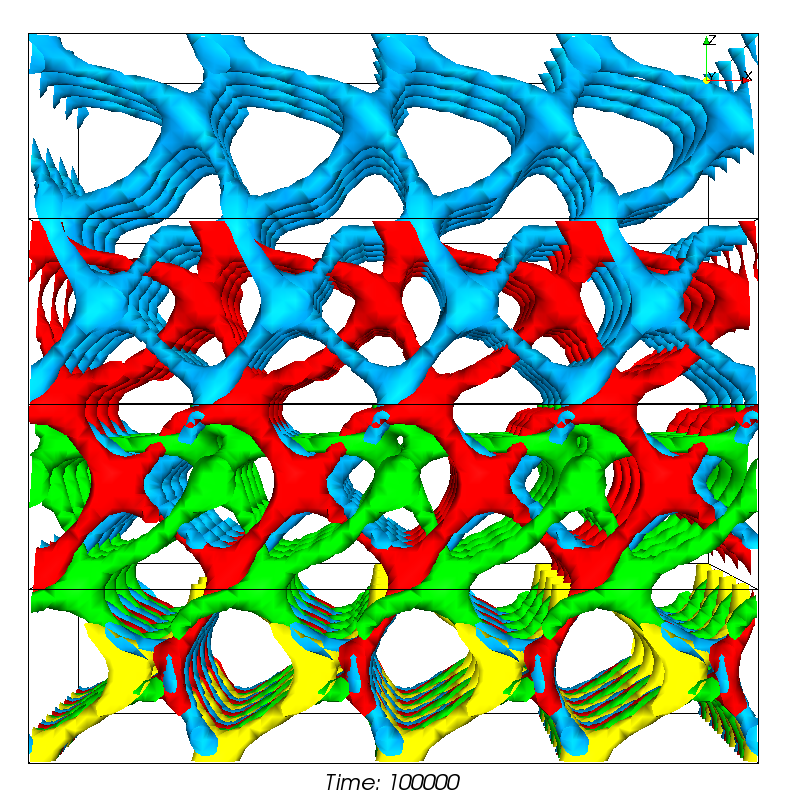
\includegraphics[width=0.245\textwidth]{disc_bp2_t-0o5_k2o0_100k.png}\\
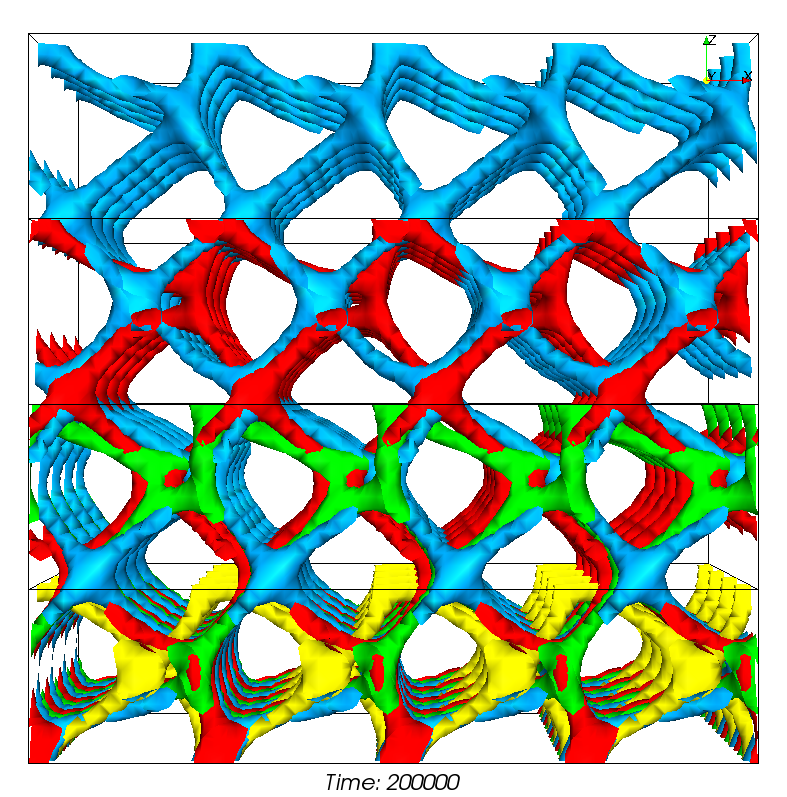
\includegraphics[width=0.245\textwidth]{disc_bp2_t-0o5_k2o0_200k.png}
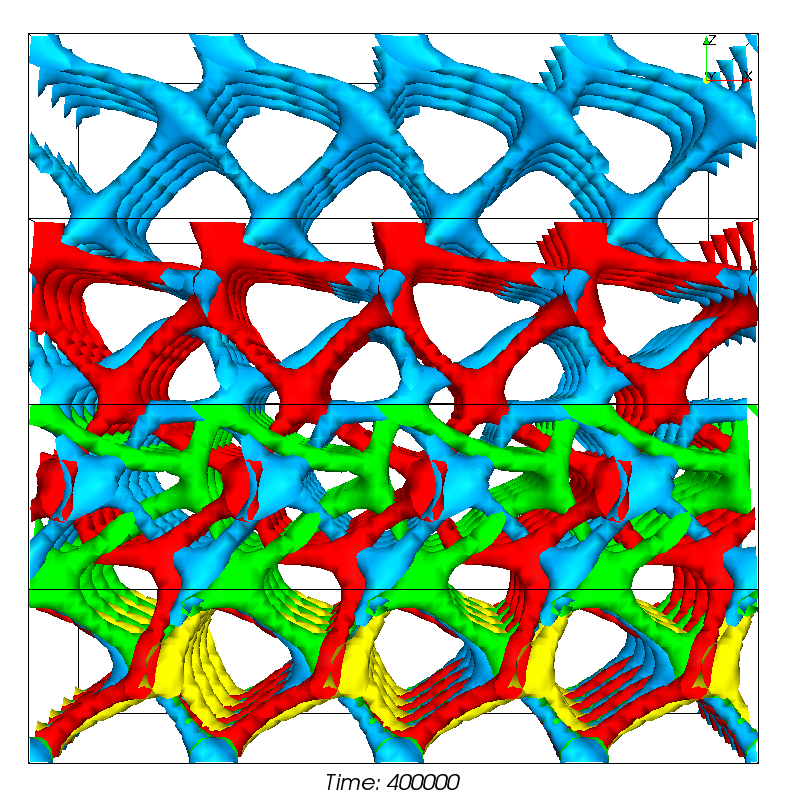
\includegraphics[width=0.245\textwidth]{disc_bp2_t-0o5_k2o0_400k.png}
\caption{}
\label{fig1}
\end{figure*}

\begin{figure*}[h]
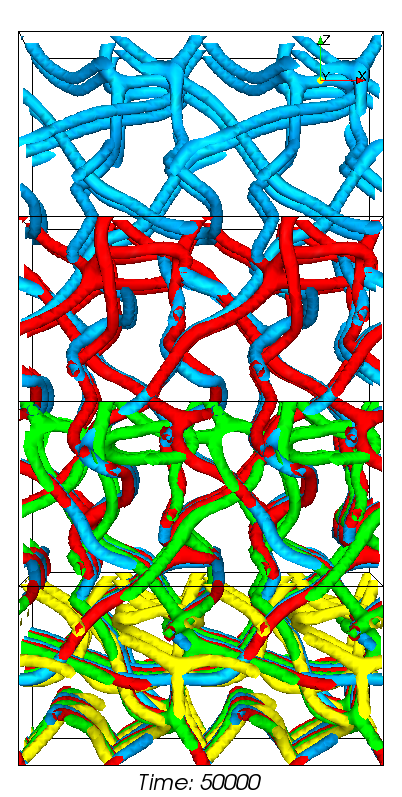
\includegraphics[width=0.245\textwidth]{disc_bp1_t-0o5_k1o0_50k.png}
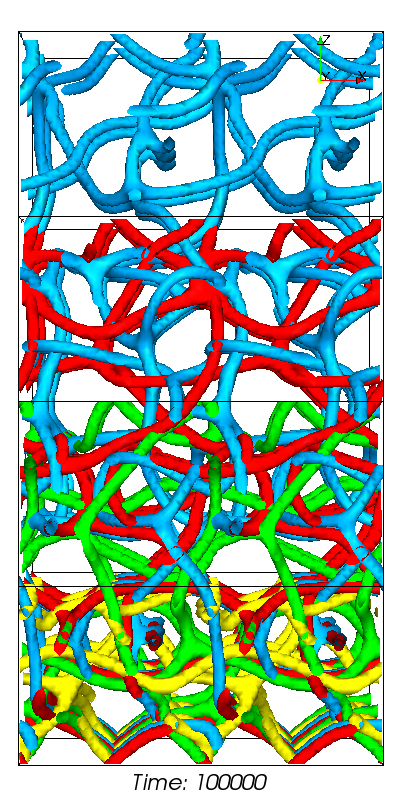
\includegraphics[width=0.245\textwidth]{disc_bp1_t-0o5_k1o0_100k.png}\\
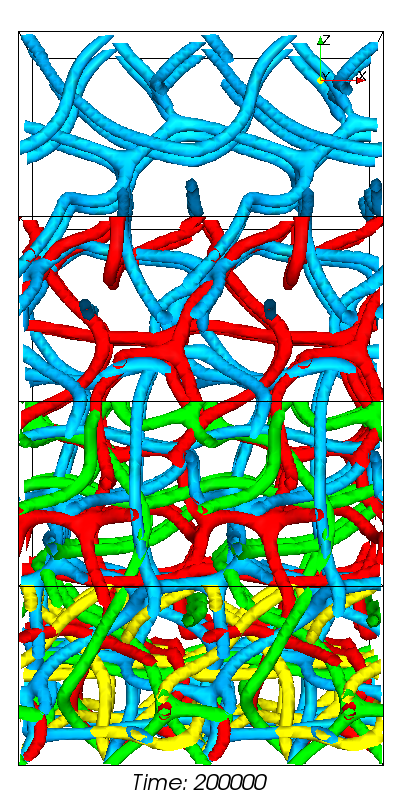
\includegraphics[width=0.245\textwidth]{disc_bp1_t-0o5_k1o0_200k.png}
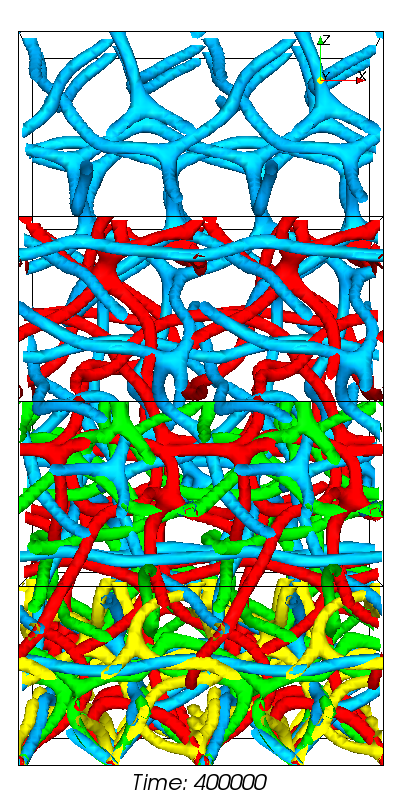
\includegraphics[width=0.245\textwidth]{disc_bp1_t-0o5_k1o0_400k.png}
\caption{}
\label{fig2}
\end{figure*}

\section{Conclusions}

% If in two-column mode, this environment will change to single-column
% format so that long equations can be displayed. Use
% sparingly.
%\begin{widetext}
% put long equation here
%\end{widetext}

% figures should be put into the text as floats.
% Use the graphics or graphicx packages (distributed with LaTeX2e)
% and the \includegraphics macro defined in those packages.
% See the LaTeX Graphics Companion by Michel Goosens, Sebastian Rahtz,
% and Frank Mittelbach for instance.
%
% Here is an example of the general form of a figure:
% Fill in the caption in the braces of the \caption{} command. Put the label
% that you will use with \ref{} command in the braces of the \label{} command.
% Use the figure* environment if the figure should span across the
% entire page. There is no need to do explicit centering.

% \begin{figure}
% \includegraphics{}%
% \caption{\label{}}
% \end{figure}

% Surround figure environment with turnpage environment for landscape
% figure
% \begin{turnpage}
% \begin{figure}
% \includegraphics{}%
% \caption{\label{}}
% \end{figure}
% \end{turnpage}

% tables should appear as floats within the text
%
% Here is an example of the general form of a table:
% Fill in the caption in the braces of the \caption{} command. Put the label
% that you will use with \ref{} command in the braces of the \label{} command.
% Insert the column specifiers (l, r, c, d, etc.) in the empty braces of the
% \begin{tabular}{} command.
% The ruledtabular enviroment adds doubled rules to table and sets a
% reasonable default table settings.
% Use the table* environment to get a full-width table in two-column
% Add \usepackage{longtable} and the longtable (or longtable*}
% environment for nicely formatted long tables. Or use the the [H]
% placement option to break a long table (with less control than 
% in longtable).
% \begin{table}%[H] add [H] placement to break table across pages
% \caption{\label{}}
% \begin{ruledtabular}
% \begin{tabular}{}
% Lines of table here ending with \\
% \end{tabular}
% \end{ruledtabular}
% \end{table}

% Surround table environment with turnpage environment for landscape
% table
% \begin{turnpage}
% \begin{table}
% \caption{\label{}}
% \begin{ruledtabular}
% \begin{tabular}{}
% \end{tabular}
% \end{ruledtabular}
% \end{table}
% \end{turnpage}

% Specify following sections are appendices. Use \appendix* if there
% only one appendix.

% If you have acknowledgments, this puts in the proper section head.
\begin{acknowledgments}
Thanks folks!
\end{acknowledgments}

% Create the reference section using BibTeX:
%\bibliography{lmc-proc}

\end{document}
%
% ****** End of file apstemplate.tex ******

